%%%%%%%%%%%%%%%%%%%%%%%%%%%%%%%%%%%%%%%%%%%%%%%%%%%%%%%%
% Canonical : https://github.com/lduran2/ece3413_classical_control_systems/doc/lab0405.tex
% Lab report
% By        : Leomar Duran <https://github.com/lduran2>
% When      : 2022-03-30t03:10Q
% For       : ECE 3413
% Version   : 1.9.0
%%%%%%%%%%%%%%%%%%%%%%%%%%%%%%%%%%%%%%%%%%%%%%%%%%%%%%%%
\documentclass[11pt]{article}
\usepackage[utf8]{inputenc}

\usepackage{lib/ccsreport}

\begin{document}

\title{ECE 3413 Lab 04/05 Time Response of First- and\\* Second-Order Systems}
\author{Leomar Durán}
\date{28\(^{\text{th}}\) March 2022}

\maketitle

\section*{Revision History}

\begin{tabularx}\linewidth{@{}rlrX@{}}
    \toprule
        Revision \#
            & Author
            & Revision date
            & Comments
    \\*
    \midrule
        1.9.0
            & Leomar Durán
            & 2022-03-30t03:10Q
            & added all models
    \\*
        1.8.0
            & Leomar Durán
            & 2022-03-30t02:05Q
            & finished adding scripts, related report
    \\*
        1.7.2
            & Leomar Durán
            & 2022-03-30t00:45Q
            & parameter scripts added to appendix
    \\*
        1.7.1
            & Leomar Durán
            & 2022-03-29t23:40Q
            & part I procedure done
    \\*
        1.7.0
            & Leomar Durán
            & 2022-03-29t22:47Q
            & rise time added to real, imaginary
    \\*
        1.6.2
            & Leomar Durán
            & 2022-03-29t22:09Q
            & rise time added to real, imaginary
    \\*
        1.6.1
            & Leomar Durán
            & 2022-03-29t21:02Q
            & clean up after real, imaginary
    \\*
        1.6.0
            & Leomar Durán
            & 2022-03-29t20:56Q
            & summary for real, imaginary
    \\*
        1.5.0
            & Leomar Durán
            & 2022-03-29t18:24Q
            & solved for real, imaginary parts
    \\*
        1.4.0
            & Leomar Durán
            & 2022-03-29t15:20Q
            & second-order peak time, overshoot
    \\*
        1.3.0
            & Leomar Durán
            & 2022-03-29t06:12Q
            & steady-state normalization, start second-order
    \\*
        1.2.0
            & Leomar Durán
            & 2022-03-29t00:05Q
            & explaining model of \(G_1(\cdot;\cdot)\)
    \\*
        1.1.0
            & Leomar Durán
            & 2022-03-28t22:09Q
            & introduction
    \\*
        1.0.0
            & Leomar Durán
            & 2022-03-28t21:39Q
            & initial lab 04/05
    \\*
        0.0.0
            & Leomar Durán
            & 2022-01-31t00:00R
            & template complete
    \\*
    \bottomrule
\end{tabularx}

\section{Introduction}

The purpose of this lab is
to evaluate the effects of poles, zeros and the gain
on first-order and second-order control systems.

After this lab, students will be able
to determine the effects of poles, zeros, and gain
as well the imaginary and real parts of poles,
and the damping ratio
on overshoot, settling time, rise time, peak time
and the overall shape of the step response.

Additionally, students will be able to plot the transient responses of systems, which include
the impulse response, step response, ramp response, and parabola response. The MATLAB \mintinline{matlab}{linearSystemAnalyzer} is also introduced as a tool for analysis.

\section{Procedure}

\begin{adjustwidth}{0.5in}{0in}
    \subsection{Part I}
        Many of the parameters for the Simulink model of Part I are calculated in MATLAB. Because of this I have included the corresponding scripts in Appendix \ref{apx:top param}--\ref{apx:last param}.

        \subsubsection{Poles in first-order systems}
        In Part I, we will practice by first performing modifications to the parametric first-order system
        \[
            G_1\brao{s; a} := \frac{a}{s + a},
        \]
        and analyze the resulting effects with the \mintinline{matlab}{linearSystemAnalyzer}.

        We will analyze \(G_1\brao{s;a}\) for \(a \in \brac{1..4}\). These systems are modelled by the Simulink subsystem in Fig. \ref{fig:1st order pole}.

        \begin{figure}
            \centering
            \includegraphics[%
                page=2,%
                trim=3.375in 2.125in 3.375in 2.0625in,%
                clip,%
                width=0.75\linewidth%
            ]{lab0405/fig/time_response_slx1.pdf}%
            \caption{Part I: Manipulating the pole in a First-Order System.}
            \label{fig:1st order pole}
        \end{figure}

        Effectively, this is manipulation of the pole of \(G_1\brao{s;a}\). The gain is also changed simultaneously to keep the steady state value at \(1\), thus normalizing with the steady state value. The steady state value is specified by \(\lim_{s\to0} G(s)\).

        Without this normalization, we would have \(G\brao{s;a} = \frac1{s + a}\), and its stead state value
        \[
            G(s) \xrightarrow{s\to0} \frac1{\brao0 + a} = \frac1a.
        \]
        Thus we divide by \(\lim_{s\to0} G(s)\) or \(\frac1a\) to normalize
        \[
            G_1\brao{s;a} = \frac{1}{s + a} \div \frac1a = \frac{a}{s + a}.
        \]

        \subsubsection{Real and imaginary parts of poles in second-order systems}

        Next in Part I, we analyze the manipulation of the poles in the second-order function
        \[
            G_2\brao{s; a,b} := \frac{b}{s^2 + as + b}
        \]
        Specifically, we will change independently the real \(x\) and imaginary \(y\) parts of the pole \(x + y\mathcal{j}\), and the natural frequency \(\omega_n\), which relates to the pole \(2\zeta\omega_n\).

        \begin{figure}
            \centering
            \includegraphics[%
                page=3,%
                trim=2.75in 2.6875in 2.75in 2.625in,%
                clip,%
                width=0.75\linewidth%
            ]{lab0405/fig/time_response_slx1.pdf}%
            \caption{Manipulating the pole in a Second-Order System \tbrao{of the real part, the imaginary part, or the natural frequency}.}
            \label{fig:2nd order pole}
        \end{figure}

        The analysis for the second-order systems in Part I, all use models with the form described in Fig. \ref{fig:2nd order pole}. However, with the values in \(G_b\) and \(G_a\) changed depending on the analysis.

        In exercises 2 and 3 respectively, we vary the real part of the pole and the imaginary part of the pole, respectively, each by multiplying it by a coefficient.

        Well, the poles of \(G_2\brao{s; a,b} = \frac{B}A\brao{s}\) have
        \[
            \begin{aligned}
                \brao*{
                    \mathfrak{Re}\Brac{s} \middle| A(s) = 0%
                    \,
                } &{}= \brao*{\frac{-a}{2}}\brac*{
                    \begin{matrix}
                        1 \\* 1 \\*
                    \end{matrix}
                },
            \\*
                \brao*{
                    \mathfrak{Im}\Brac{s} \middle| A(s) = 0%
                    \,
                } &{}= \brao*{\sqrt{b - \brao*{\frac{a}2}^2}}\brac*{
                    \begin{matrix}
                        1 \\* -1 \\*
                    \end{matrix}
                }.
            \\*
            \end{aligned}
        \]

        Now let \(
            k, l \in \mathbb{C},
            \setprime{A} : \mathbb{C} \to \mathbb{C}
        \), s.t.
        \(
            \brao*{\mathfrak{Re}\Brac{s} \middle| \setprime{A}\brao{s} = 0} = k\brao*{\mathfrak{Re}\Brac{s} \middle| A\brao{s} = 0}
        \),
        \(
            \brao*{\mathfrak{Im}\Brac{s} \middle| \setprime{A}\brao{s} = 0} = l\brao*{\mathfrak{Im}\Brac{s} \middle| A\brao{s} = 0}
        \),
        then
        \newcommand*\realimaginarypoles{%
            \[
                \setprime{{\vec{s}\,{\vphantom{1^1}}}}
                := \brao*{s \middle| \setprime{A}\brao{s} = 0}
                = \brac*{
                    \begin{matrix}
                        1 & \mathcal{j} \\* 1 & -\mathcal{j} \\*
                    \end{matrix}
                }\brac*{
                    \begin{matrix}
                        k\brao*{\frac{-a}{2}} \\*
                        l\sqrt{b - \brao*{\frac{a}2}^2}
                        \\*
                    \end{matrix}
                }.
            \]%
        }%
        \realimaginarypoles
        These are the roots of \(
            s^2 + kas + \brao*{l^2 b + \brao*{k^2 - l^2}\brao*{\frac{a}2}^2}
        \).

        \paragraph{Peak time}

        % Note that:
        %
        % The roots of s^2 + (2zw)s + w^2 are
        %   s1, s2
        % = (-2zw +/- sqrt(4w^2 - (2zw)^2))/2
        % = -zw +/- sqrt(4w^2 - 4z^2 w^2)/2
        % = -zw +/- 2w sqrt(1 - z^2)/2
        % = -zw +/- w sqrt(1 - z^2)
        %
        % So   Re{s}  = -zw
        % and |Im{s}| = w sqrt(1 - z^2)

        Then the new peak time for \(s \in \setprime{\mathbf{s}}\),
        \[
            \setprime{T}_p
            := \frac\pi{\abs{\mathfrak{Im}\Brac{s}}}
            = \frac\pi{l\sqrt{b - \brao*{\frac{a}2}^2}}
            = \frac{1}l \brao*{\frac\pi{\sqrt{b - \brao*{\frac{a}2}^2}}}
            = \frac{T_p}l.
        \].

        We see that the coefficient of the real part \(k\) has no effect on the peak time. However, the coefficient of the imaginary part \(l\) is inversely proportional to peak time.

        \paragraph{Overshoot}
        Now the new overshoot
        \[
                \setprime{OS}
                := \exp\brao*{\pi\brao*{\frac{\mathfrak{Re}}{\abs{\mathfrak{Im}}}}\Brac{s}}
                = \exp\brao*{\brao\pi\frac
                    {k\brao*{\frac{-a}2}}
                    {l\sqrt{b - \brao*{\frac{a}2}^2}}
                }
                = \exp\brao*{\frac{k}l\brao*{\brao\pi\frac
                    {\brao*{\frac{-a}2}}
                    {\sqrt{b - \brao*{\frac{a}2}^2}}
                }}
        \]
        is necessary and sufficient for
        \[
            \ln\brao{\setprime{OS}} = \frac{k}l\ln\brao*{OS}.
        \]
        Thus we see that \(\hfrac{k}l\) is proportional to the logarithm of the overshoot.

        \paragraph{Constraint for settling time}

        % The polynomial with roots s = x +/- yj, where x = Re{s} and y = |Im{s}|
        %
        %   (s - x - yj)(s - x + yj)
        % = (s - x)^2 - (yj)^2
        % = (s - x)^2 + y^2
        % = s^2 - 2xs + (x^2 + y^2)
        % = s^2 + (2zw)s + w^2
        % 
        % So  w = sqrt(x^2 + y^2) = sqrt(Re^2{s} + Im^2{s})
        % and z = -x/w = -Re{s}/w

        Next the settling time
        \[
            T_s
            := \frac{\ln\brao*{\SI2\percent \sqrt{1 - \zeta^2}}}{\mathfrak{Re}\Brac{s}}.
        \]

        Well, let's assume, \(T_s\) is a normal distribution with the approximation
        \[
            \widehat{T_s}
            := \frac{\ln\brao{\SI2\percent}}{\mathfrak{Re}\Brac{s}}.
        \]
        For all \(\zeta \in \brac*{0,1}\), the rate of error for this approximation
        \[
             \frac{T_s - \widehat{T_s}}{T_s}
             = -\brao*{\frac{2\ln\brao{\SI2\percent}}{\ln\brao*{1 - \zeta^2}} + 1}^{-1}
             < 0.
        \]
        So, the error is in the right tail of the distribution. An outlier in a normal distribution is approximated as a value \(1.5\) standard deviations from the mean. We expect a proportion \(0.9332\) of data is within this range. Thus, we find a \(\max\Brac\zeta\) satisfying
        \[
            \frac{T_s - \widehat{T_s}}{T_s}
            \leq \num{0.9332} - 1
            < 0.
        \]
        This \(\max\Brac\zeta \approx \num{0.654847}\), which gives a settling time with an error within \(\SI{6.68}\percent\).

        Now generally
        \[
            \begin{aligned}
                \omega_n
                    &{}:= \sqrt{\mathfrak{Re}^2\Brac{s} + \abs{\mathfrak{Im}}^2\Brac{s}},
            \\*
                \zeta
                    &{}:= \frac{-\mathfrak{Re}\Brac{s}}{\omega_n}.
            \\*
            \end{aligned}
        \]

        So we have
        \[
            \begin{aligned}
                \setprime{\omega}_n
                    &{}= \sqrt{k^2 \mathfrak{Re}^2\Brac{s} + l^2 \abs{\mathfrak{Im}}^2\Brac{s}},
            \\*
                \setprime\zeta
                    &{}= \frac{-k\mathfrak{Re}\Brac{s}}{\omega_n}
                    = \frac{1}{\sqrt{1 + \brao*{
                        \frac{l}k
                        \brao*{\frac
                            {\abs{\mathfrak{Im}}}
                            {\mathfrak{Re}}
                        }
                        \Brac{s}
                    }^2}}.
            \\*
            \end{aligned}
        \]

        Thus, we choose coefficients \(k, l\) s.t.
        \[
            \frac{l}k
            \geq \frac{\sqrt{\frac1{\zeta^2} - 1}}{\brao*{\mathfrak{\abs{Im}/Re}}\Brac{s}}
            = \frac{\sqrt{\frac1{\brao{\num{0.654847}}^2} - 1}}{\brao*{\mathfrak{\abs{Im}/Re}}\Brac{s}}
            = \frac
                {-1.154104}
                {\brao*{\mathfrak{\abs{Im}/Re}}\Brac{s}}.
        \]

        Given our system \(G_2\brao{s; a, b}\), where we have
        \(a = 4\) and \(b = 25\), then \(
            \mathfrak{Re}\Brac{s} = -4/2 = -2
        \) and \(
            \abs{\mathfrak{Im}}\Brac{s} = \sqrt{25 - \brao{4/2}^2} = \sqrt{21}
        \). Thus \(\frac{l}k \geq \num{0.503692}\).

        For fixed \(l = 1\),
        then \(k \leq {2.0}\),
        whereas for fixed \(k = 1\),
        then \(l \geq {0.50}\).

        We will be be using fixed \(l = 1\)
        and \(k \in \brao{1, 2, 1/2}\),
        each of the latter of which fulfills \(k \leq 2.0\).
        Then we will use fixed \(k = 1\)
        and \(l \in \brao{1, 2, 4}\),
        each of the latter of which fulfills \(l \geq 0.50\). Thus, the constraint of \(\max\Brac\zeta \approx \num{0.654847}\) is met.

        \paragraph{Settling time}
        Thus, we can use the approximation \(\widehat{T_s}\) as a stand-in for \(T_s\). Therefore
        \[
            \widehat{\setprime{T}_s}
            := \frac{\ln\brao{\SI2\percent}}{k\mathfrak{Re}\Brac{s}}
            = \frac1k \brao*{\frac{\ln\brao{\SI2\percent}}{\mathfrak{Re}\Brac{s}}}
            = \frac{\widehat{T_s}}k.
        \]

        Thus the coefficient of the imaginary part of the poles \(l\) has no effect on settling time.
        However, the coefficient of the real part \(k\) is inversely proportional to settling time.

        \paragraph{Rise time}
        In the case of the rise time generally,
        \[
            T_r
            :=
                \frac{\ln\brao*{\SI{90}\percent \sqrt{1 - \zeta^2}}}{\mathfrak{Re}\Brac{s}}
                - \frac{\ln\brao*{\SI{10}\percent \sqrt{1 - \zeta^2}}}{\mathfrak{Re}\Brac{s}}.
            = \frac{\ln\brao*{\frac
                {\SI{90}\percent}
                {\SI{10}\percent}
            }}{\mathfrak{Re}\Brac{s}}.
        \]
        So there is no need for approximation. The new rise time
        \[
            \setprime{T}_r
            := \frac{\ln\brao*{\frac
                {\SI{90}\percent}
                {\SI{10}\percent}
            }}{k \mathfrak{Re}\Brac{s}}
            = \frac1k \brao*{\frac{\ln\brao*{\frac
                {\SI{90}\percent}
                {\SI{10}\percent}
            }}{\mathfrak{Re}\Brac{s}}}
            = \frac{T_r}{k}
        \]

        However, like with settling time,
        the coefficient of the real part of the poles is inversely proportional to the rise time.

        \paragraph{Summary}
        Given coefficients \(k, l \in \mathbb{C}\)
        for the real and imaginary parts of the poles respectively,
        we have the following relations
        \begin{eqnarray}
            \llap{\(
                \setprime{T}_p
            \)} = \rlap{\(
                \dfrac{T_p}l,
            \)}
        \\*
            \llap{\(
                \ln\brao{\setprime{OS}}
            \)} = \rlap{\(
                \dfrac{k}l\ln\brao*{OS},
            \)}
        \\*
            \llap{\(
                \widehat{\setprime{T}_s}
            \)} = \rlap{\(
                \dfrac{\widehat{T_s}}k,
            \)}
        \\*
            \llap{\(
                \setprime{T}_r
            \)} = \rlap{\(
                \dfrac{T_r}k.
            \)}
        \end{eqnarray}

        That is, the coefficient of the imaginary part \(l\) is inversely proportional to the peak time \(\setprime{T}_p\),
        the ratio \(\frac{k}l\) is proportional to overshoot \(\setprime{OS}\),
        and the real part \(k\) is inversely proportional to both
        the approximation of the settling time \(\setprime{T}_s\)
        and the rise time \(\setprime{T}_r\).

        \subsubsection{Natural frequency of poles in second-order systems}

        Like in the previous section,
        we use Fig. \ref{fig:2nd order pole}
        for the model for varying natural frequency.

        Well it is also the case that
        \(
            A\Brac{s}
            = s^2 + 2\zeta\omega_n + \omega_n^2
        \). Thus
        \[
            \begin{aligned}
                \brao*{\mathfrak{Re}\Brac{s} \middle| A\brao{s} = 0}
                &{}= \brao{-\zeta\omega_n} \brac*{
                    \begin{matrix} 1 \\* 1\\* \end{matrix}
                },
            \\*
                \brao*{\mathfrak{Im}\Brac{s} \middle| A\brao{s} = 0}
                &{}= \brao*{\omega_n\sqrt{1 - \zeta^2}}
                \brac*{
                    \begin{matrix} 1 \\* -1\\* \end{matrix}
                },
            \\*
            \end{aligned}
        \]

        Well, let \(m \in \mathbb{C}, \setprime[2]A : \mathbb{C} \to \mathbb{C}\), s.t. the modified natural frequency \(\setprime[2]\omega_n = m\omega_n\). Then
        \newcommand*\naturalfrequencypoles{%
            \[
                \setprime[2]{{\vec{s}\,{\vphantom{1^1}}}}
                := \brao*{s \middle| \setprime[2]{A}\brao{s} = 0}
                = \brac*{
                    \begin{matrix}
                        1 & \mathcal{j} \\* 1 & -\mathcal{j} \\*
                    \end{matrix}
                }\brao*{m\omega_n}\brac*{
                    \begin{matrix}
                        -\zeta \\*
                        \sqrt{1 - \zeta^2}
                        \\*
                    \end{matrix}
                }.
            \]%
        }%
        \naturalfrequencypoles
        These are the roots of \(s^2 + 2\zeta\brao*{m\omega_n} + \brao*{m\omega_n}^2\).

        \paragraph{Peak time}

        Then the new peak time for \(s \in \setprime{\mathbf{s}}\),
        \[
            \setprime[2]{T}_p
            := \frac\pi{\abs{\mathfrak{Im}\Brac{s}}}
            = \frac\pi{-\zeta\brao{m\omega_n}}
            = \frac1m \brao*{\frac\pi{-\zeta\omega_n}}
            = \frac{T_p}m.
        \].

        \paragraph{Overshoot}
        Now the new overshoot
        \[
                \setprime[2]{OS}
                := \exp\brao*{\pi\brao*{\frac{\mathfrak{Re}}{\abs{\mathfrak{Im}}}}\Brac{s}}
                = \exp\brao*{\brao*\pi\frac
                    {-\zeta\brao*{m\omega_n}}
                    {\brao*{m\omega_n} \sqrt{1 - z^2}}
                }
                = \brao*{\exp\brao*{\brao*\pi\frac
                    {-\zeta\omega_n}
                    {\omega_n \sqrt{1 - z^2}}
                }}
                = OS.
        \]

        \paragraph{Settling time}
        Next the settling time
        \[
            \setprime[2]{T}_s
            := \frac{\ln\brao*{\SI2\percent \sqrt{1 - \zeta^2}}}{\mathfrak{Re}\Brac{s}}
            = \frac{\ln\brao*{\SI2\percent \sqrt{1 - \zeta^2}}}{-\zeta\brao{m\omega_n}}
            = \frac1m\brao*{\frac{\ln\brao*{\SI2\percent \sqrt{1 - \zeta^2}}}{-\zeta\omega_n}}
            = \frac{T_s}m.
        \]

        \paragraph{Rise time}
        Finally the rise time
        \[
            \setprime[2]T_r
            := \frac{\ln\brao*{\frac
                {\SI{90}\percent}
                {\SI{10}\percent}
            }}{\mathfrak{Re}\Brac{s}}
            = \frac{\ln\brao*{\frac
                {\SI{90}\percent}
                {\SI{10}\percent}
            }}{-\zeta\brao{m\omega_n}}
            = \frac1m\brao*{
                \frac{\ln\brao*{\frac
                    {\SI{90}\percent}
                    {\SI{10}\percent}
                }}{-\zeta\omega_n}
            }
            = \frac{T_r}m.
        \]

        \paragraph{Summary}
        With the natural frequency, its coefficient is inversely proportional to peak time, settling time and rise time. However, it has no effect on the overshoot.

        \subsubsection{Linear analysis}
        The linear analysis is performed
        using a REPL-style program
        available in \ref{apx:linear analysis}.
        This allows the user to choose
        any of the systems modeled in this lab
        and view its linear analysis.

        Additionally, the overshoot, settling time, peak time and rise time are recorded in the Results.

        \subsubsection{Pole locations}
        To find the pole locations, we use the script in Appendix \ref{apx:part 01 pz map}.
        However formulas for the poles have been described earlier in rectangular form and are provided again for convenience with the original poles.

        \[
            \vec{s}
            := \brao*{s \middle| A\brao{s} = 0}
            = \brac*{
                \begin{matrix}
                    1 & \mathcal{j} \\* 1 & -\mathcal{j} \\*
                \end{matrix}
            }\brac*{
                \begin{matrix}
                    \brao*{\frac{-a}{2}} \\*
                    \sqrt{b - \brao*{\frac{a}2}^2}
                    \\*
                \end{matrix}
            }
            =\brac*{
                \begin{matrix}
                    1 & \mathcal{j} \\* 1 & -\mathcal{j} \\*
                \end{matrix}
            }\omega_n\brac*{
                \begin{matrix}
                    -\zeta \\*
                    \sqrt{1 - \zeta^2}
                    \\*
                \end{matrix}
            }.
        \]%

        \realimaginarypoles
        \naturalfrequencypoles

    \subsection{Part II}
    For Part II, we use MATLAB to create the transient response plots and the pole-zero map.
    The script is included in Appendix \ref{apx:part 03 transient responses}.

    \subsection{Part III}
    Many of the parameters for the Simulink model of Part I are calculated in MATLAB. Because of this I have included the corresponding scripts in Appendix \ref{apx:top param}--\ref{apx:last param}.

        \subsubsection{Added Poles}

        \begin{figure}
            \centering
            \includegraphics[%
                page=6,%
                trim=1.625in 2.125in 1.75in 2.0625in,%
                clip,%
                width=0.75\linewidth%
            ]{lab0405/fig/time_response_slx1.pdf}%
            \caption{Adding poles to a system.}
            \label{fig:adding poles}
        \end{figure}

        \subsubsection{Added Zeros}

        \begin{figure}
            \centering
            \includegraphics[%
                page=7,%
                trim=1.375in 1.25in 1.4375in 1.25in,%
                clip,%
                width=0.85\linewidth%
            ]{lab0405/fig/time_response_slx1.pdf}%
            \caption{Adding zeros to a system.}
            \label{fig:adding zeros}
        \end{figure}

        \subsubsection{Parametric Transfer Function I}

        \begin{figure}
            \centering
            \includegraphics[%
                page=8,%
                trim=0.8125in 1.3125in 0.875in 1.3125in,%
                clip,%
                width=0.9\linewidth%
            ]{lab0405/fig/time_response_slx1.pdf}%
            \caption{System with parameters for zeros, poles and gain.}
            \label{fig:parametric 1}
        \end{figure}

        \subsubsection{Parametric Transfer Function II}

        \begin{figure}
            \centering
            \includegraphics[%
                page=9,%
                trim=0.125in 1.4375in 0.1875in 1.375in,%
                clip,%
                width=\linewidth%
            ]{lab0405/fig/time_response_slx1.pdf}%
            \caption{System with parameters for zeros, poles and gain.}
            \label{fig:parametric 1}
        \end{figure}

        \subsubsection{Linear analysis}
        The linear analysis is performed
        using a REPL-style program
        available in \ref{apx:linear analysis}.
        This allows the user to choose
        any of the systems modeled in this lab
        and view its linear analysis.

        Additionally, the overshoot, settling time, peak time and rise time are recorded in the Results.

\end{adjustwidth}

\section{Results}
\section{Discussion}

\newpage
\appendix
\title{Appendix}\label{doc:apx}
\maketitle

\section{Codes and Commands used in the lab}

\begin{enumerate}
    \item
        \mintinline{matlab}{conv}
        \tabto{1.5in}
        \(\Rightarrow\) convolve or multiply polynomials
\end{enumerate}

\section{Top-level script to calculate parameters}\label{apx:top param}
\inputminted{matlab}{lab0405/programs/time_response_params_m1.m}

\section{Script to calculate variable real part pole in Part I}
\inputminted{matlab}{lab0405/programs/part0102_reals_m1.m}

\section{Script to calculate variable imaginary part pole in Part I}
\inputminted{matlab}{lab0405/programs/part0103_imags_m1.m}

\section{Script to calculate variable natural frequency in Part I}
\inputminted{matlab}{lab0405/programs/part0104_nat_freqs_m1.m}

\section{Script to calculate parameters for parametric system in Part III}\label{apx:last param}
\inputminted{matlab}{lab0405/programs/part03_params_m1.m}

\section{Script for linear analysis of systems}\label{apx:linear analysis}
\inputminted{matlab}{lab0405/programs/lin_analysis_m1.m}

\section{Script for finding the poles for the systems in Part I}\label{apx:part 01 pz map}
\inputminted{matlab}{lab0405/programs/part01_poles_zeros_m1.m}

\section{Script for finding the transient responses in Part II}\label{apx:part 03 transient responses}
\inputminted{matlab}{lab0405/programs/part02_transient_response_m1.m}

\section{Function for converting systems to symbolic expressions}
\inputminted{matlab}{lab0405/programs/sys2sym.m}

\end{document}
